%  Chapter 6

\chapter{PERFORMANCE ANALYSIS}

In this chapter we discuss the results obtained across the 3 phases of our experimentation done as a part of this project.
\begin{itemize}
    \item \textbf{Phase 1} Covers the baseline scores obtained on all tracks
    \item \textbf{Phase 2} Covers   the results obtained by performing Transfer Learning between tracks within the same level and across levels.
    \item \textbf{Phase 3} The final phase of our project covers the result obtained by training the agents in the presence of the adversaries we have devised and the results obtained by transferring the knowledge learnt from these models.
\end{itemize}

For all these phases, we present the graphs obtained during the training of our models. The first graphs shows the cumulative reward obtained during the training process and our objective is to \textit{maximise} the reward obtained. The second graphs shows the average length of an episode of agent as the training progresses. Having a lower value is \textit{better} but is not mandatory as this is an indicator of how stable the agent is with sudden dips indicating crashes on the track.

\section{PHASE I - BASELINE PERFORMANCE}
\subsection{Oval Track - Basic Track}
\begin{figure}[H]
    \centering
    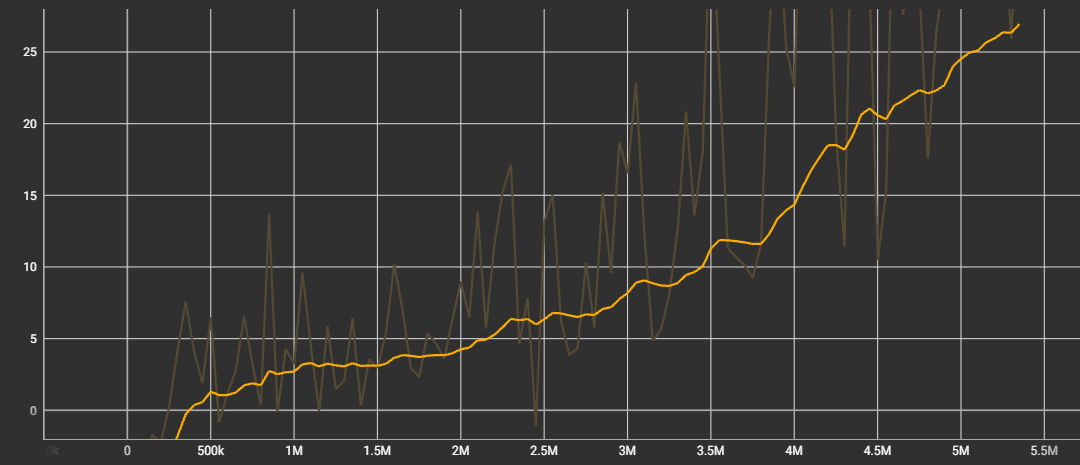
\includegraphics[width=1.0\textwidth]{images/graphs/OvalTrack-Reward.png}
    \caption{\centering Oval Track Cumulative Reward. \\ X-axis: Time steps \\ Y-axis: Cumulative Reward}
    \label{fig:rl}
\end{figure}
\begin{figure}[H]
    \centering
    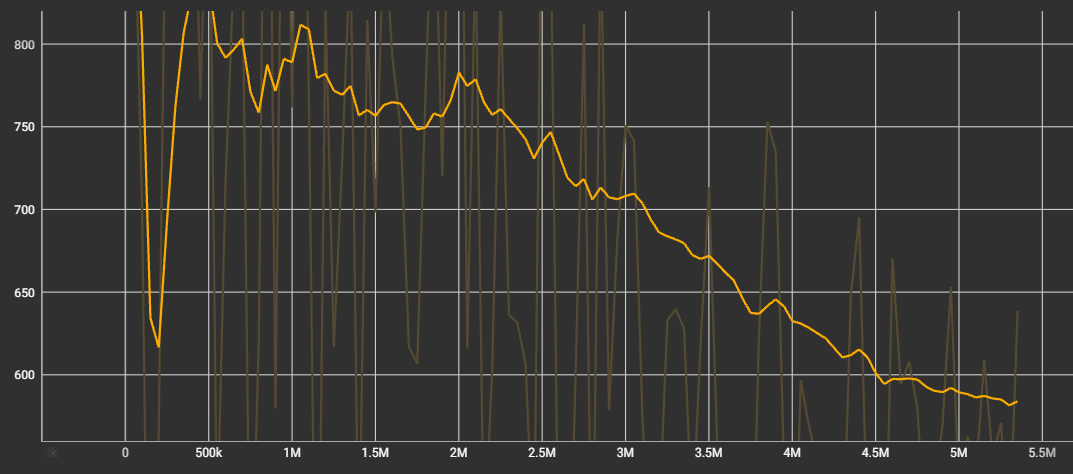
\includegraphics[width=1.0\textwidth]{images/graphs/OvalTrack-Episode.png}
    \caption{\centering Oval Track Episode Length. \\ X-axis: Time steps \\ Y-axis: Episode Length}
    \label{fig:rl}
\end{figure}


\subsection{One Kink Track}

\begin{figure}[H]
    \centering
    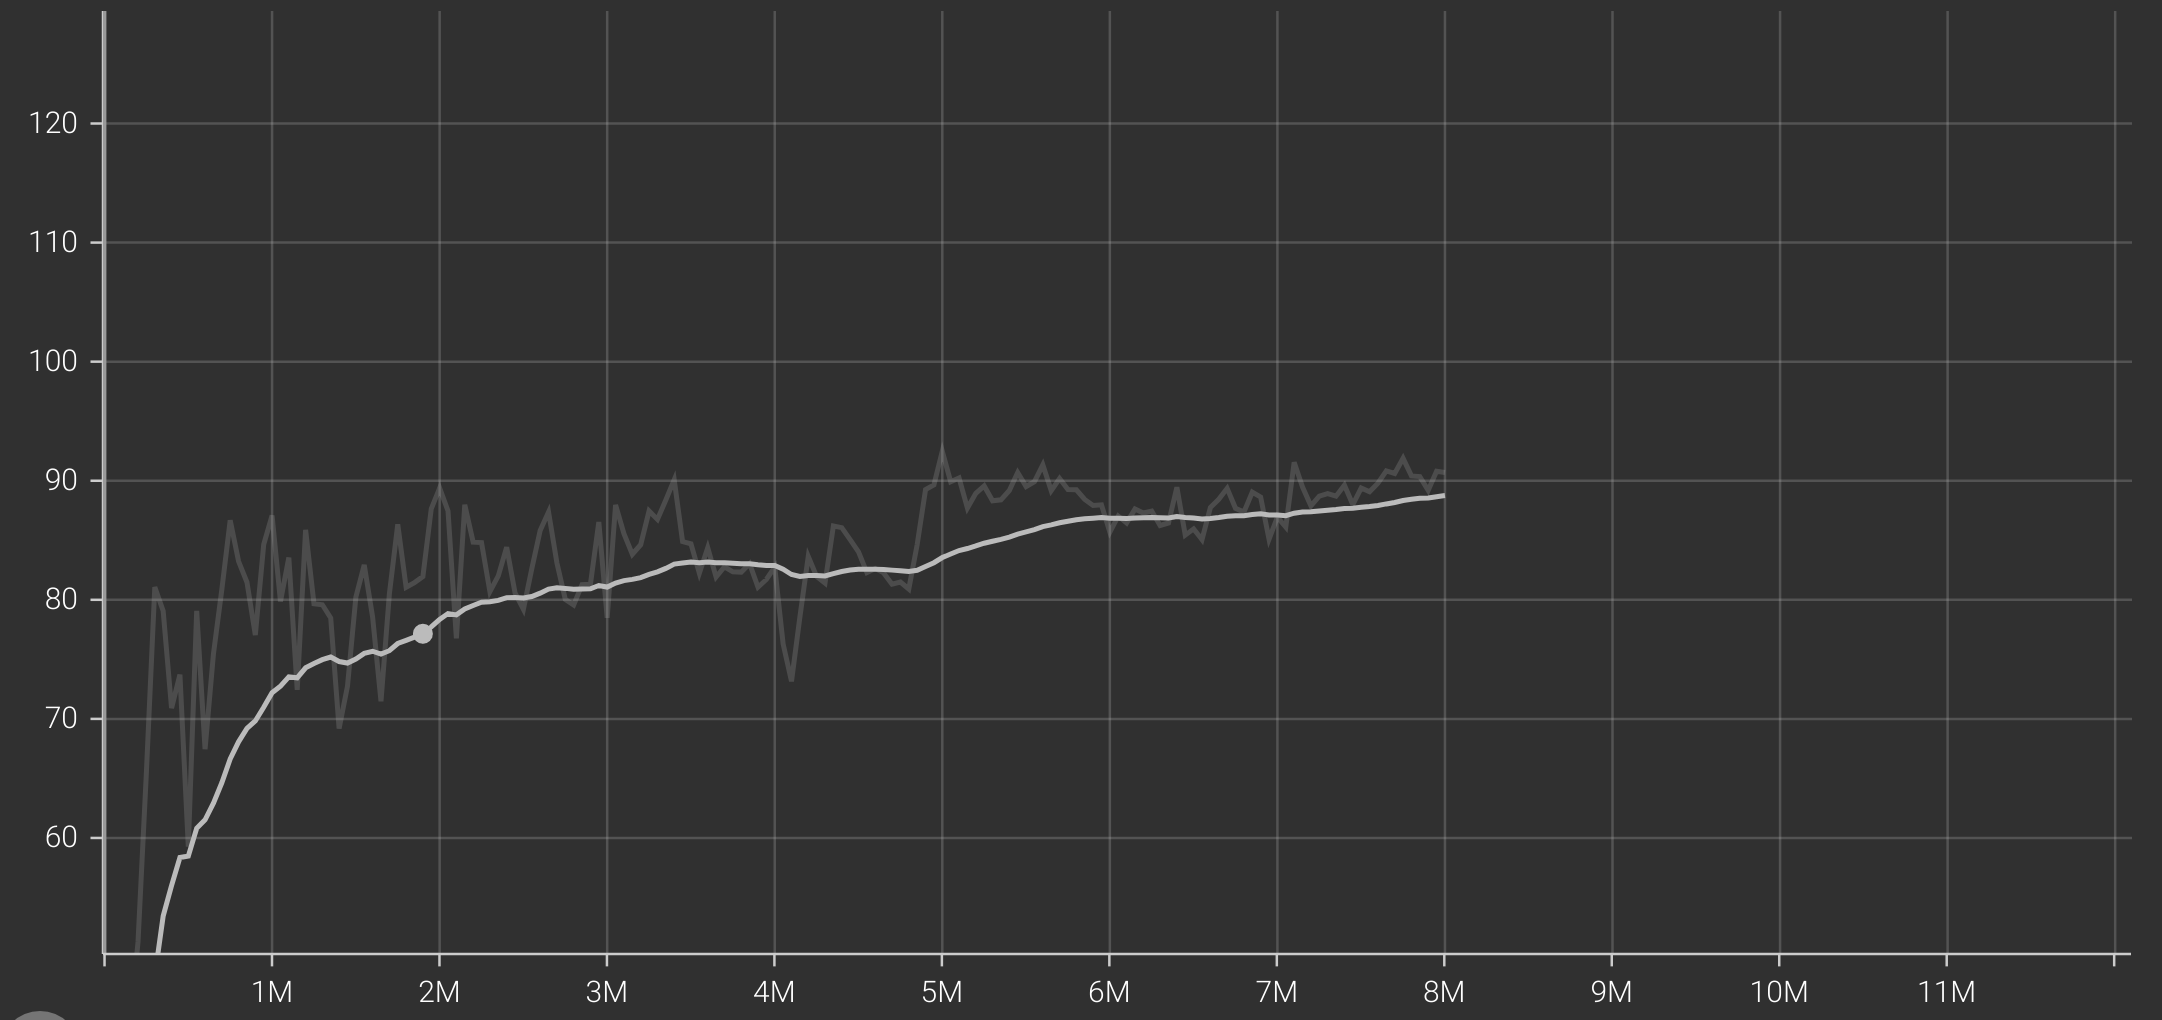
\includegraphics[width=1.0\textwidth]{images/graphs/OneKink-Reward.png}
    \caption{\centering One Kink Track Cumulative Reward. \\ X-axis: Time steps \\ Y-axis: Cumulative Reward}
    \label{fig:rl}
\end{figure}

\begin{figure}[H]
    \centering
    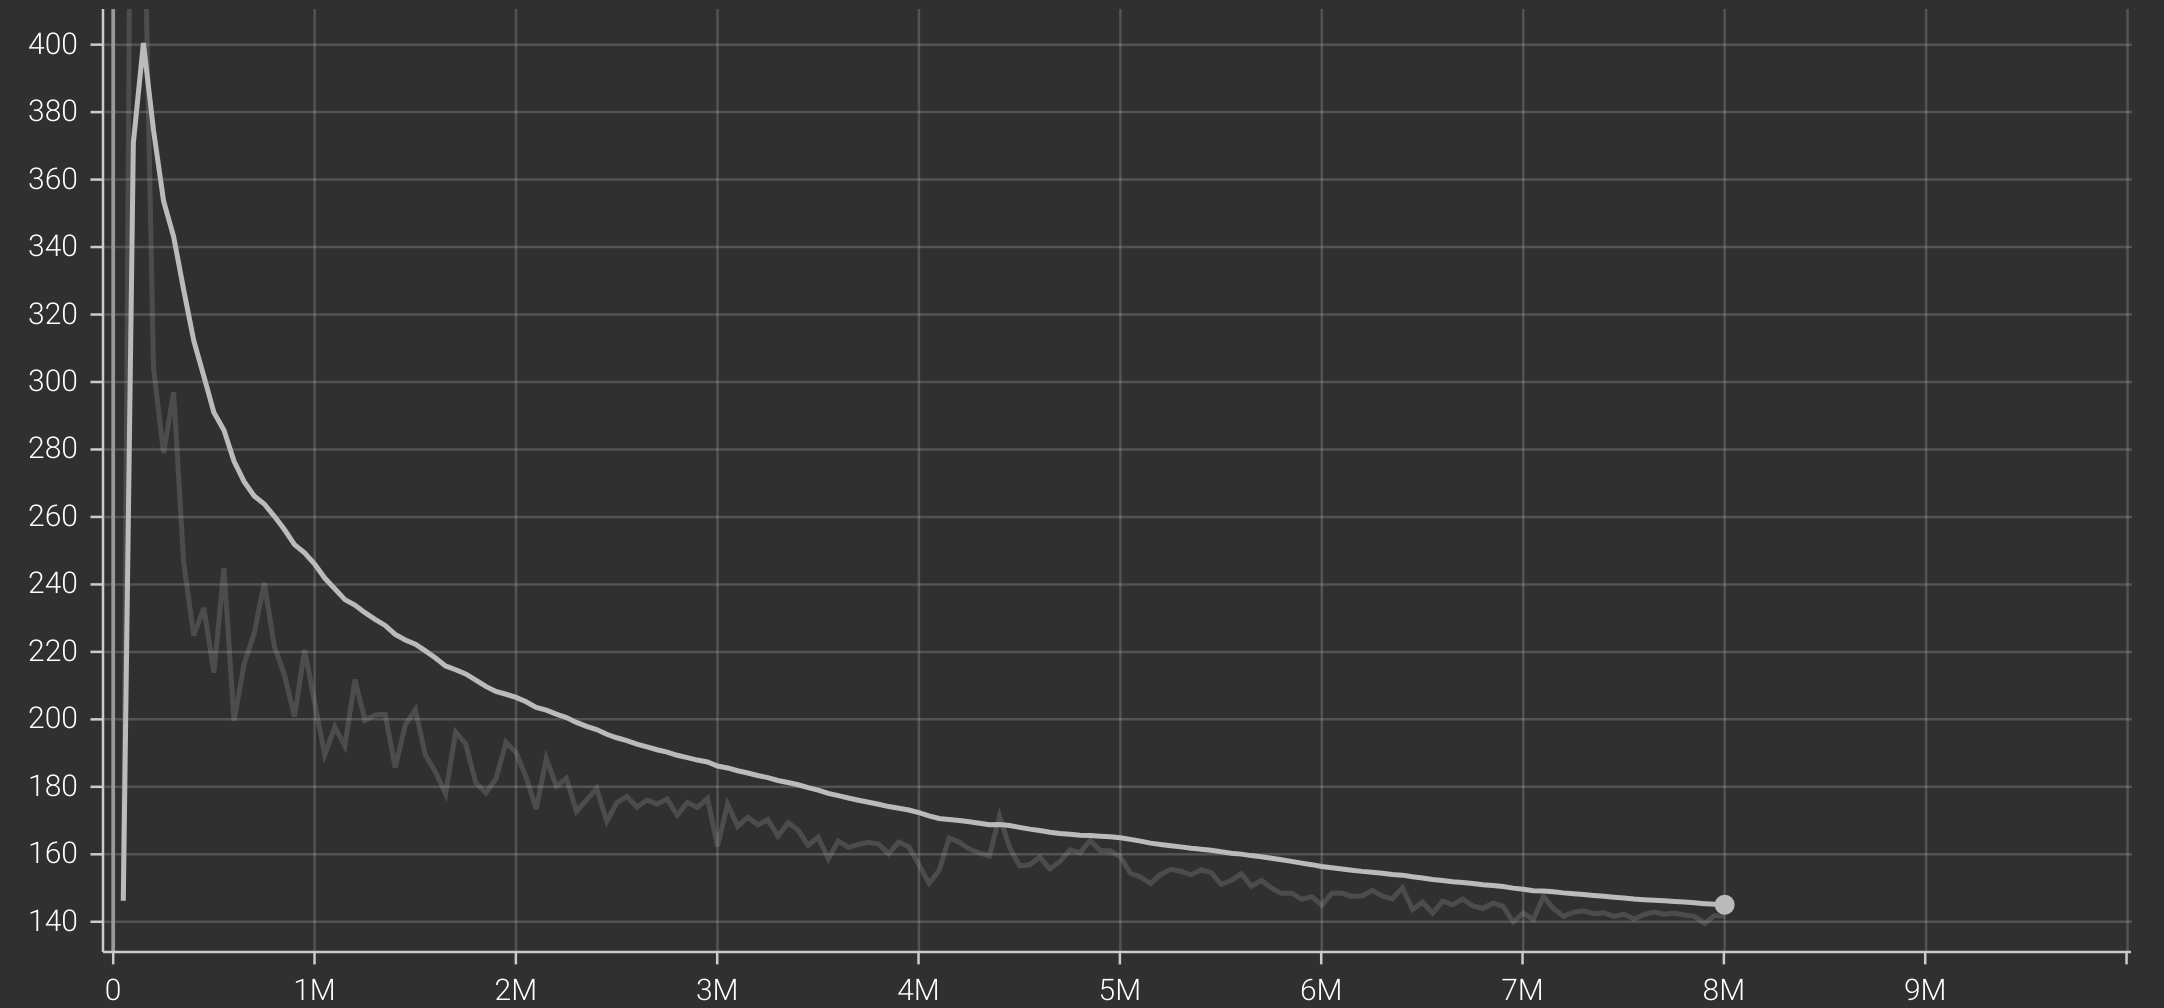
\includegraphics[width=1.0\textwidth]{images/graphs/OneKink-Episode.png}
    \caption{\centering One Kink Track Episode Length. \\ X-axis: Time steps \\ Y-axis: Episode Length}
    \label{fig:rl}
\end{figure}



\subsection{Two Kink Track}

\begin{figure}[H]
    \centering
    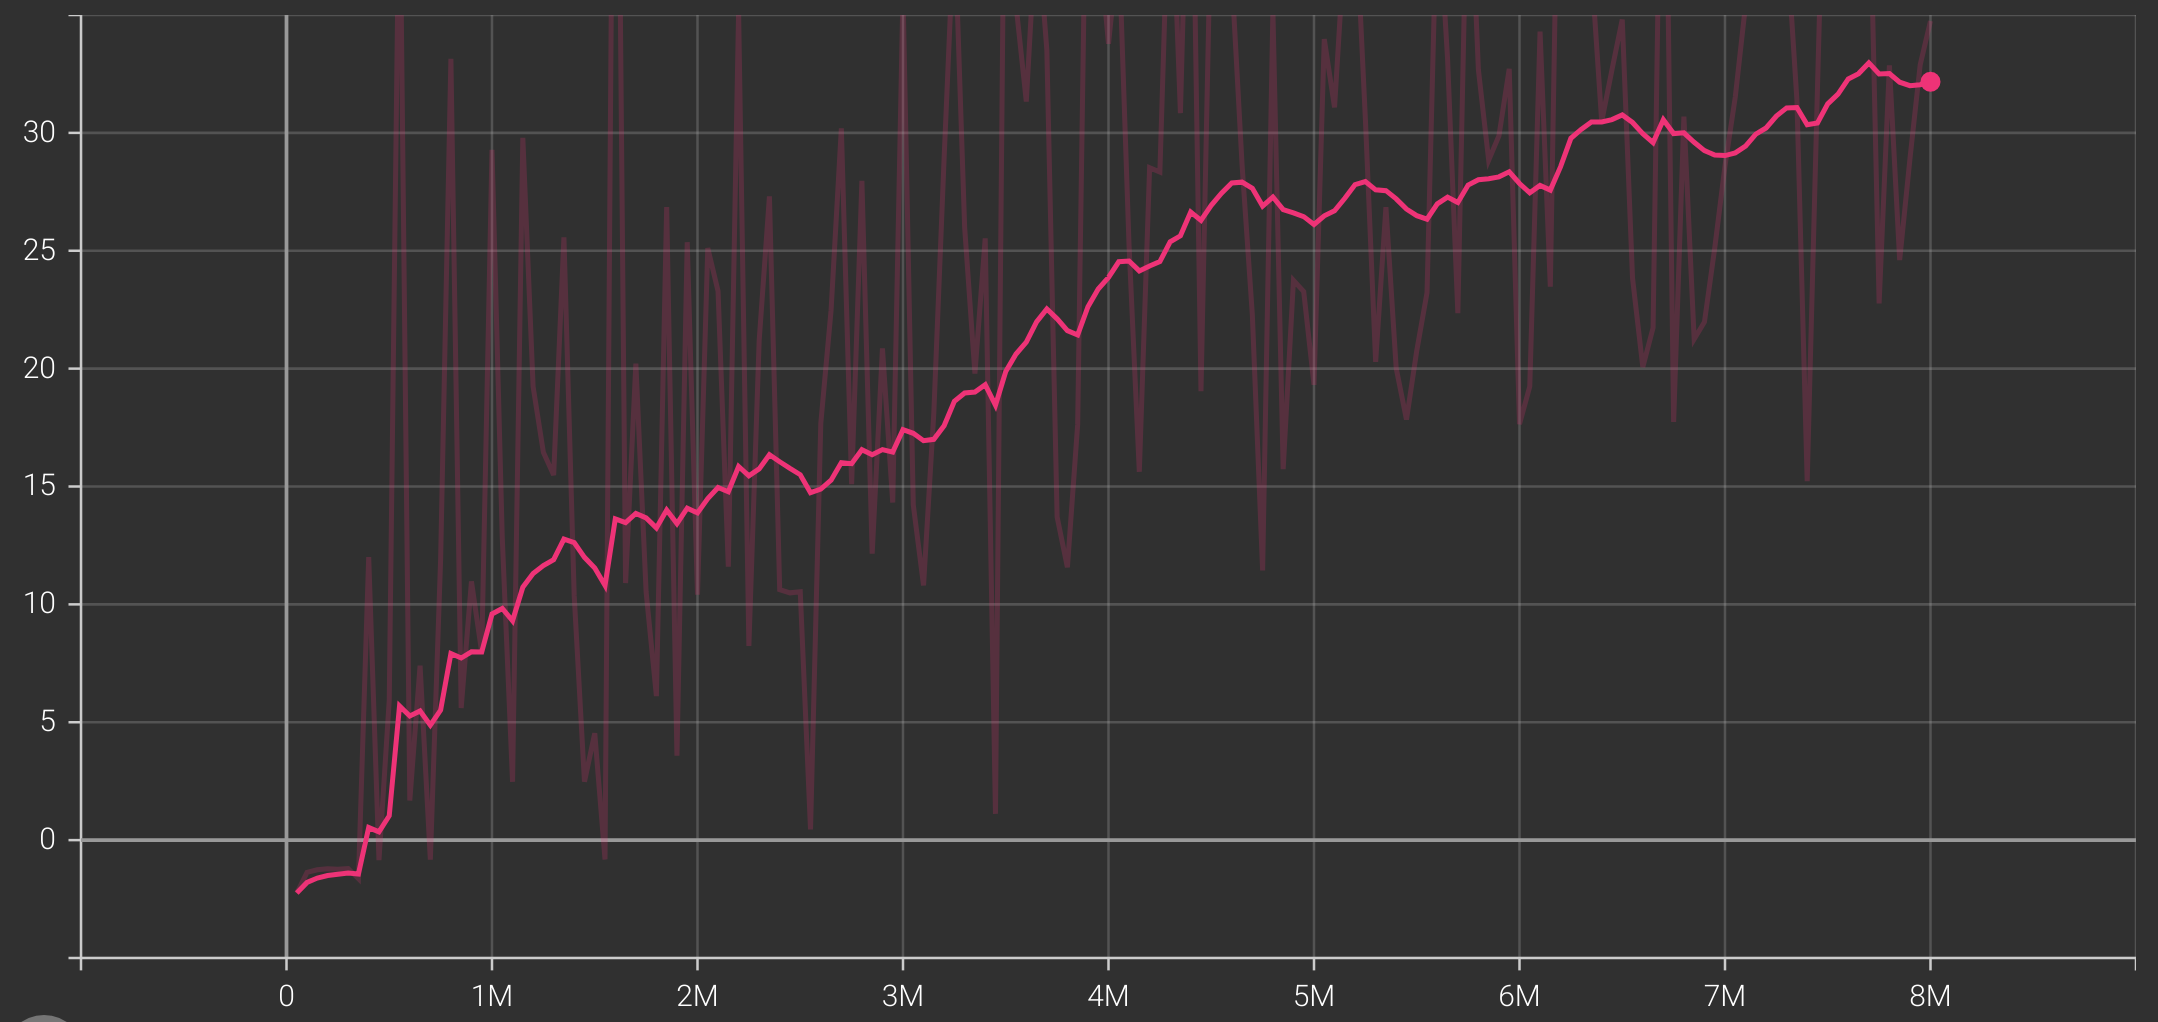
\includegraphics[width=1.0\textwidth]{images/graphs/TwoKink-Reward.png}
    \caption{\centering Two Kink Track Cumulative Reward. \\ X-axis: Time steps \\ Y-axis: Cumulative Reward}
    \label{fig:rl}
\end{figure}

\begin{figure}[H]
    \centering
    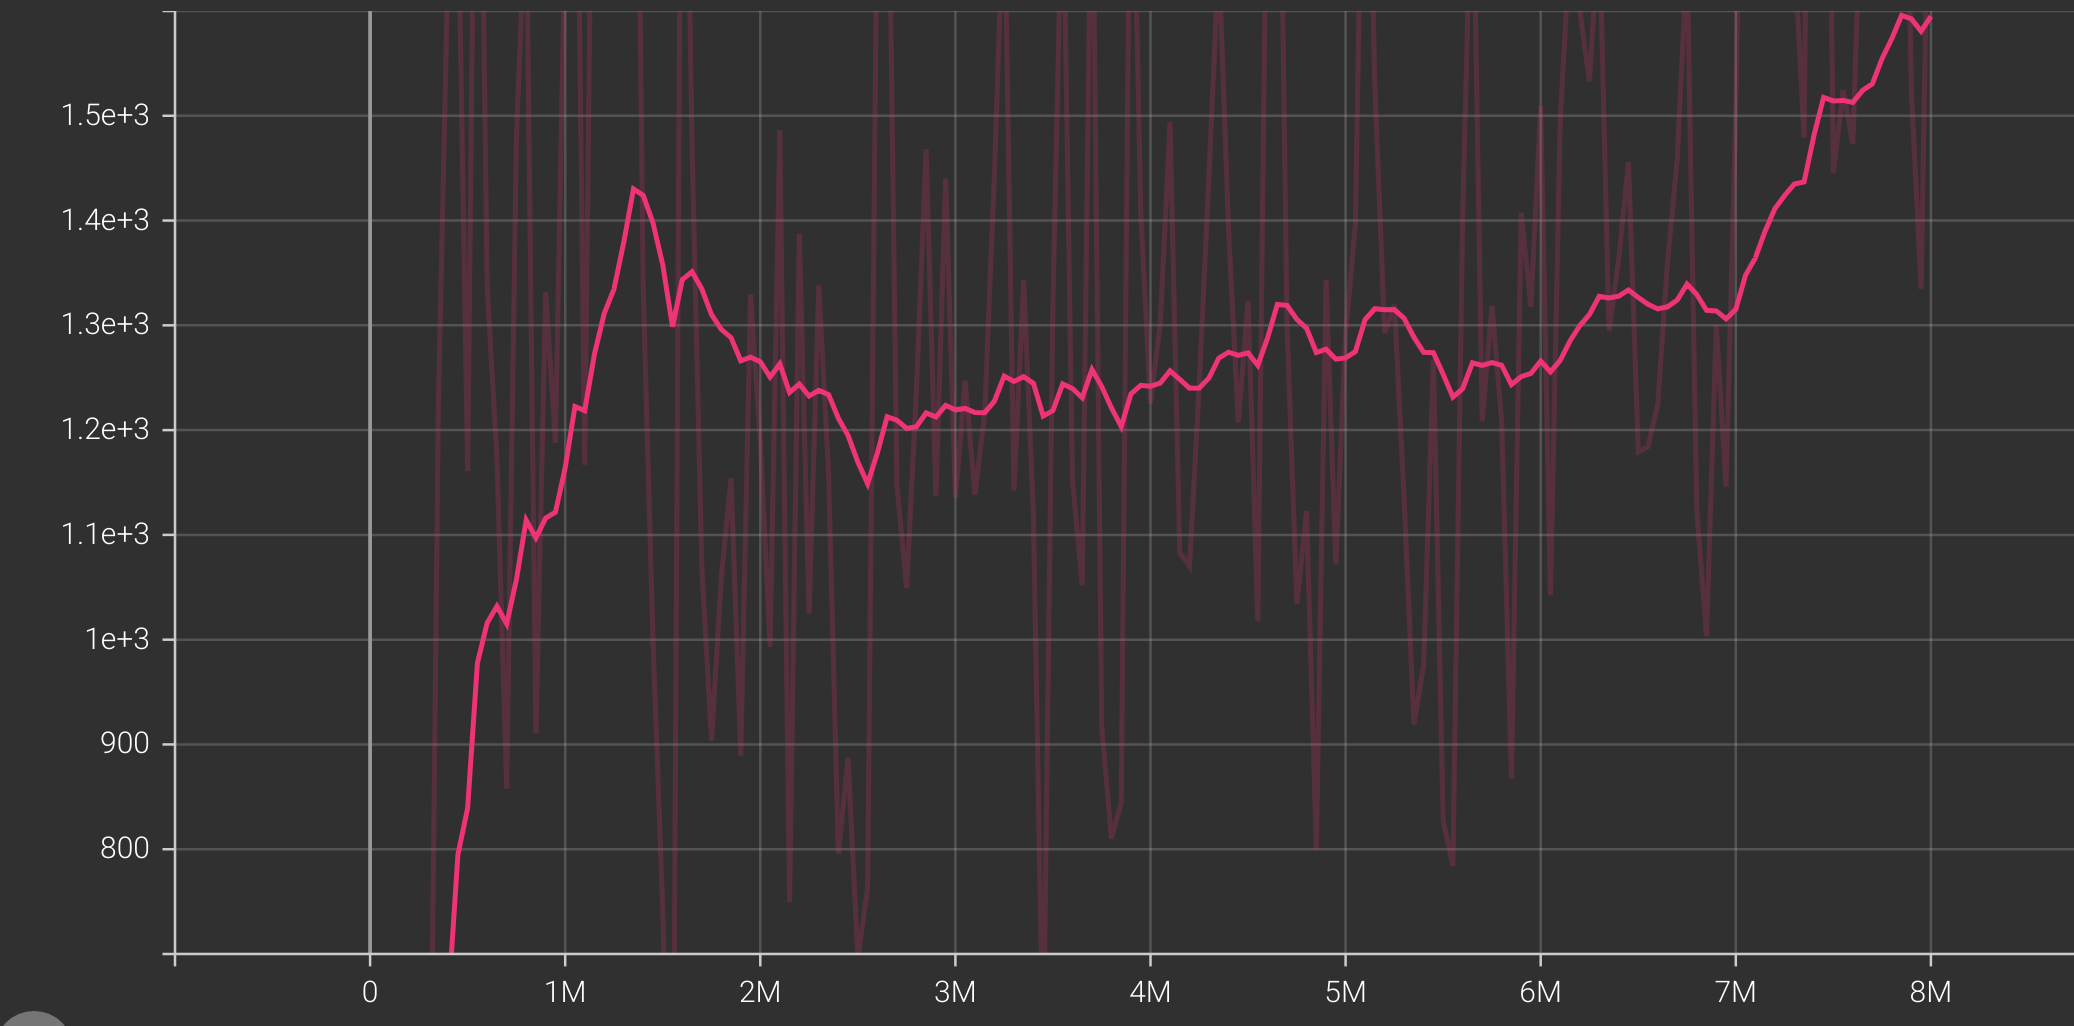
\includegraphics[width=1.0\textwidth]{images/graphs/TwoKink-Episode.png}
    \caption{\centering Two Kink Track Episode Length. \\ X-axis: Time steps \\ Y-axis: Episode Length}
    \label{fig:rl}
\end{figure}





\subsection{Barcelona}

\begin{figure}[H]
    \centering
    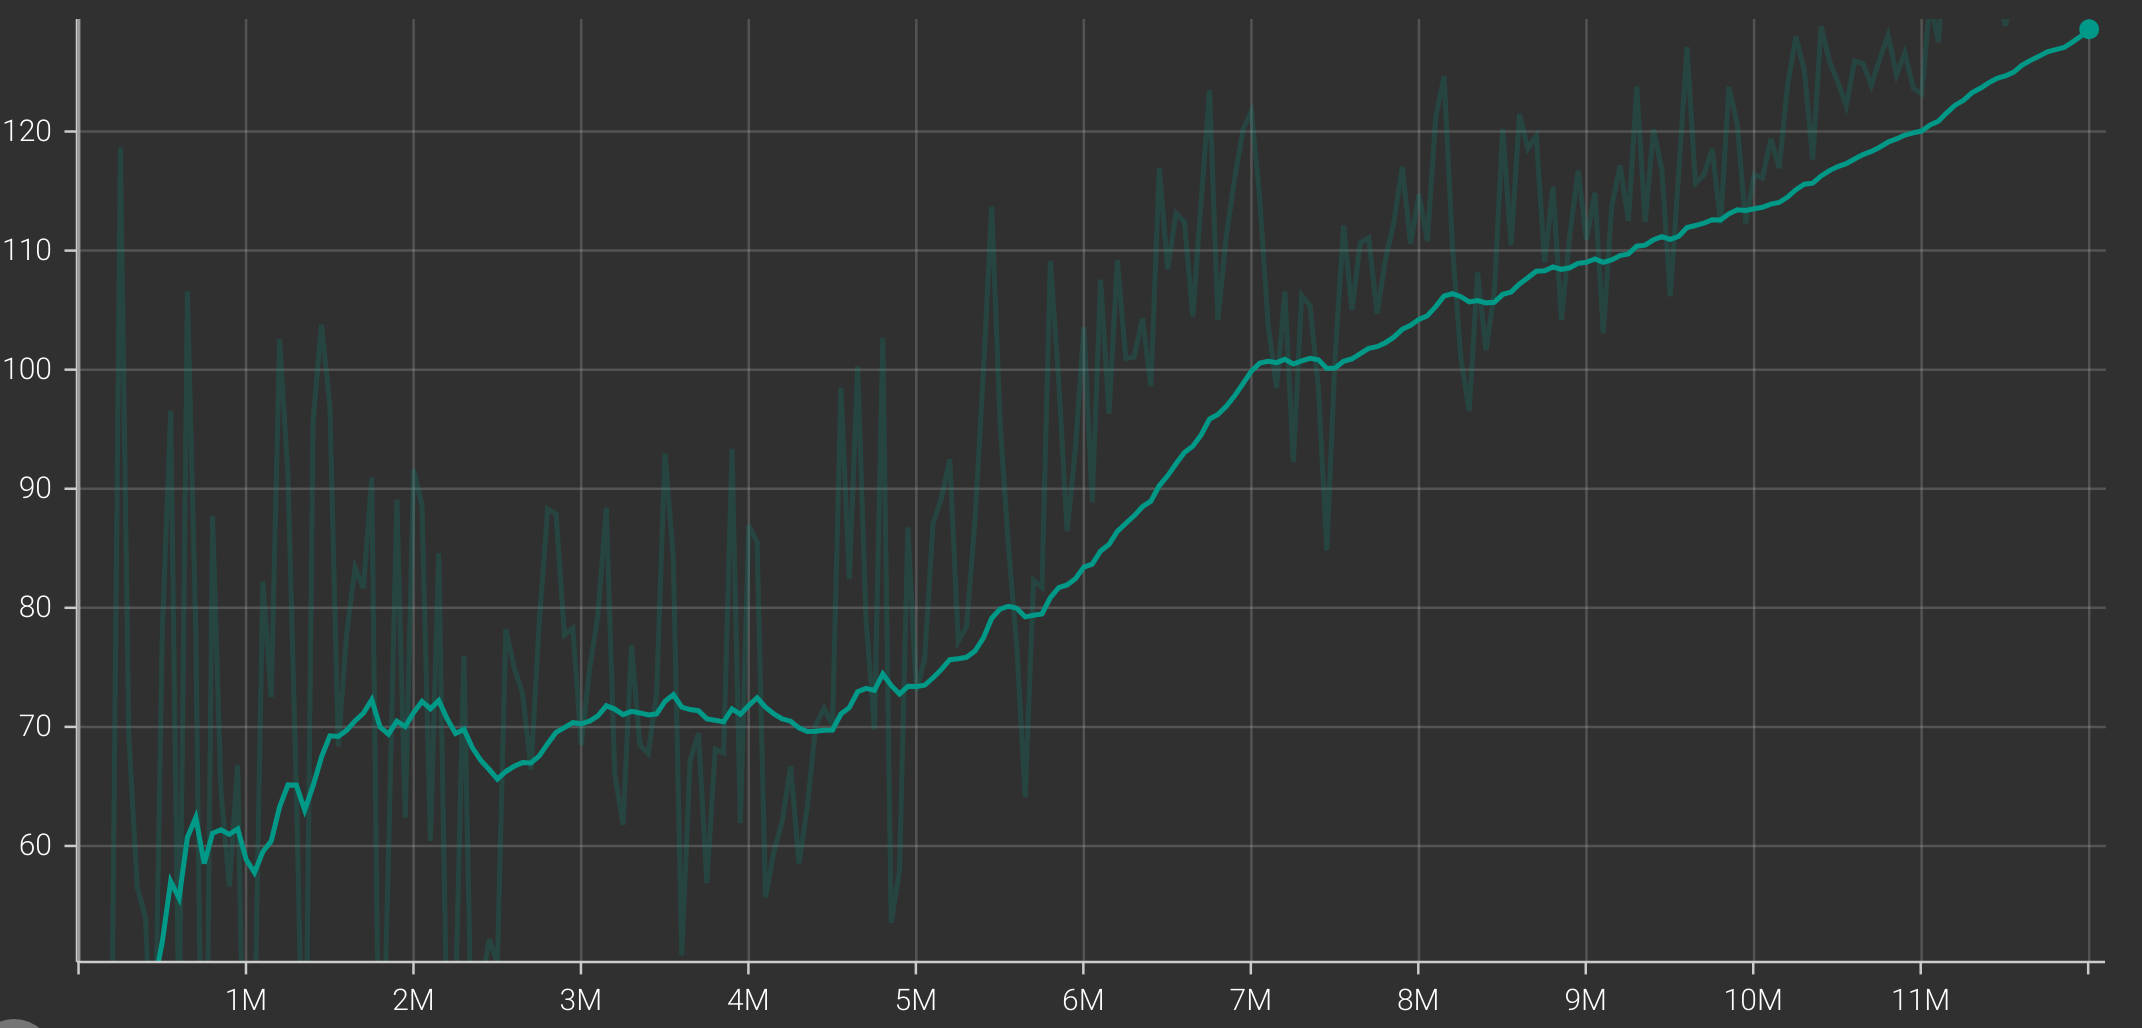
\includegraphics[width=1.0\textwidth]{images/graphs/Barcelona-Reward.png}
    \caption{\centering Barcelona Track Cumulative Reward. \\ X-axis: Time steps \\ Y-axis: Cumulative Reward}
    \label{fig:rl}
\end{figure}

\begin{figure}[H]
    \centering
    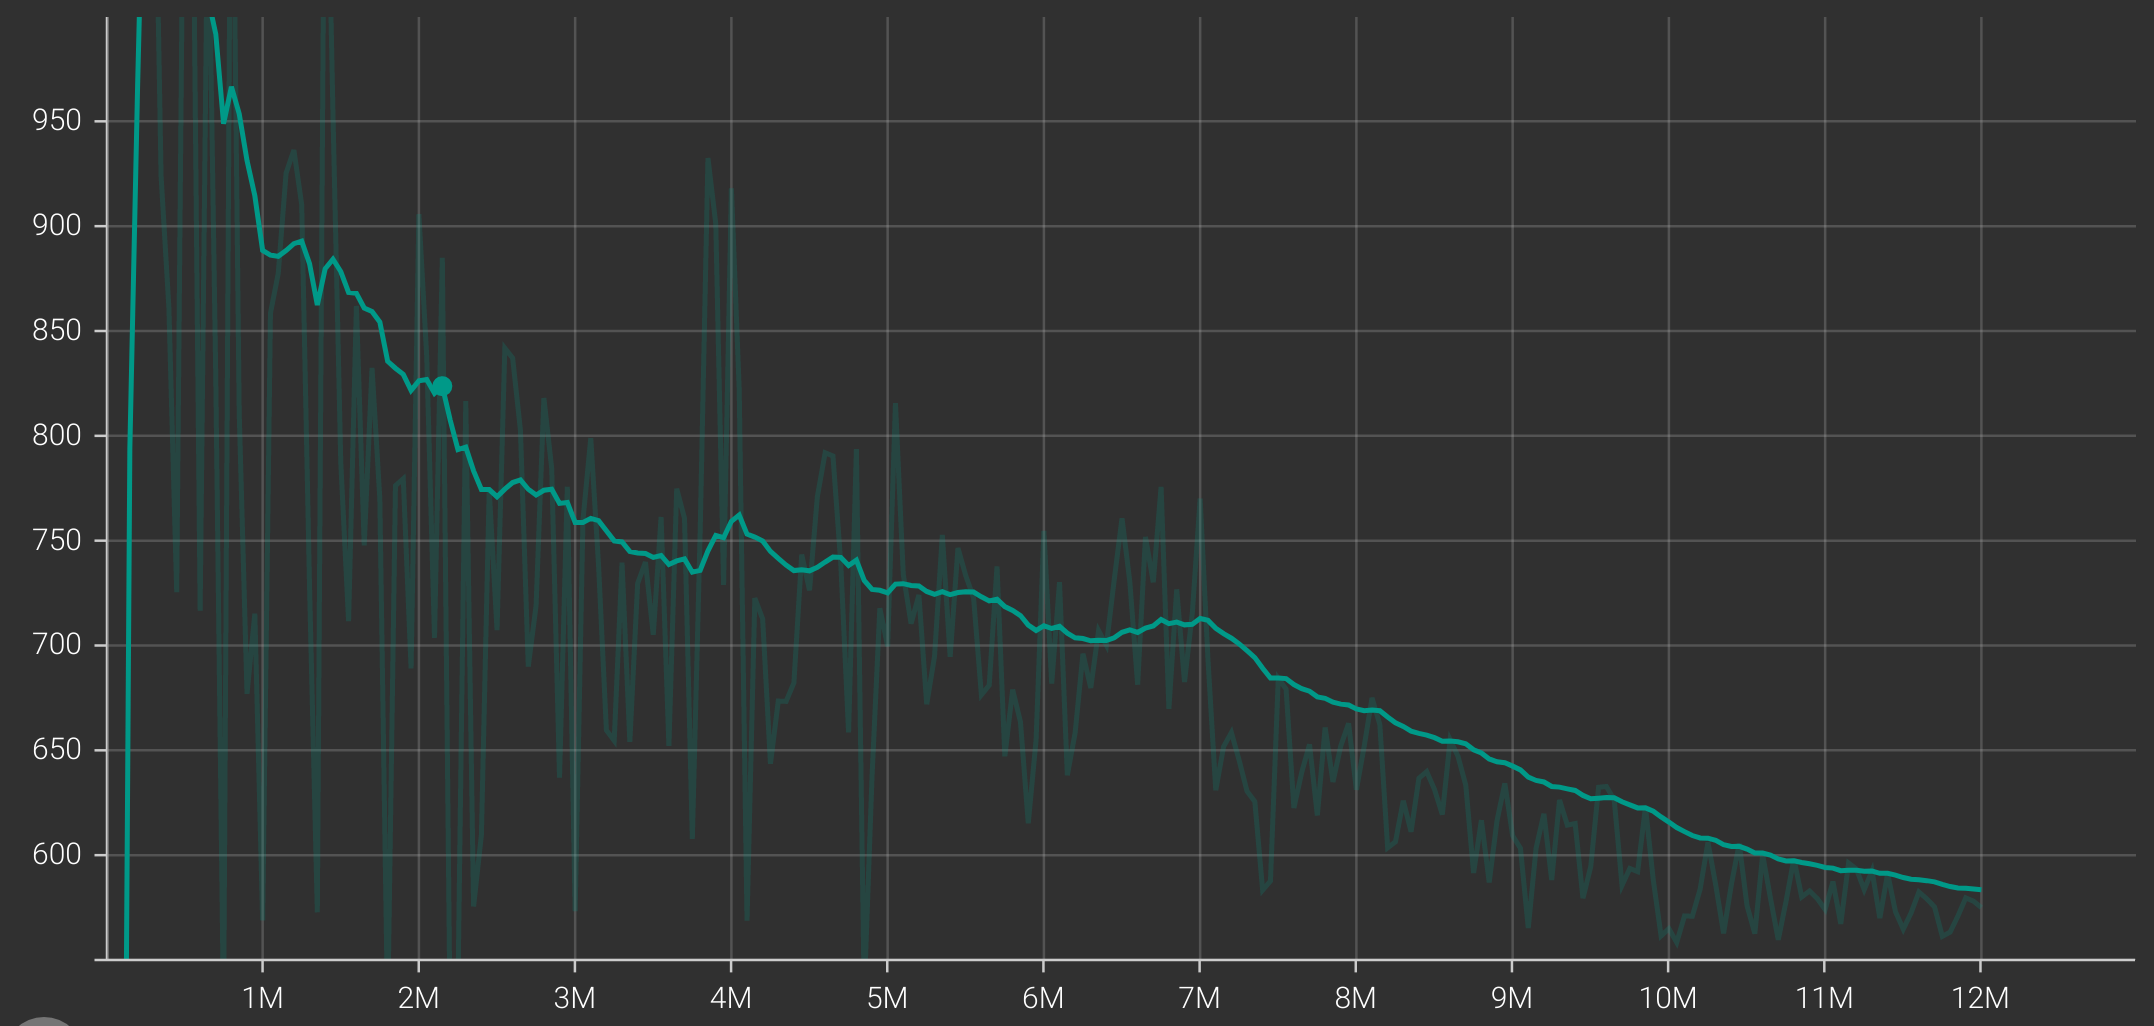
\includegraphics[width=1.0\textwidth]{images/graphs/Barcelona-Episode.png}
    \caption{\centering Barcelona Track Episode Length. \\ X-axis: Time steps \\ Y-axis: Epsiode Length}
    \label{fig:rl}
\end{figure}

\subsection{AWS Track}

\begin{figure}[H]
    \centering
    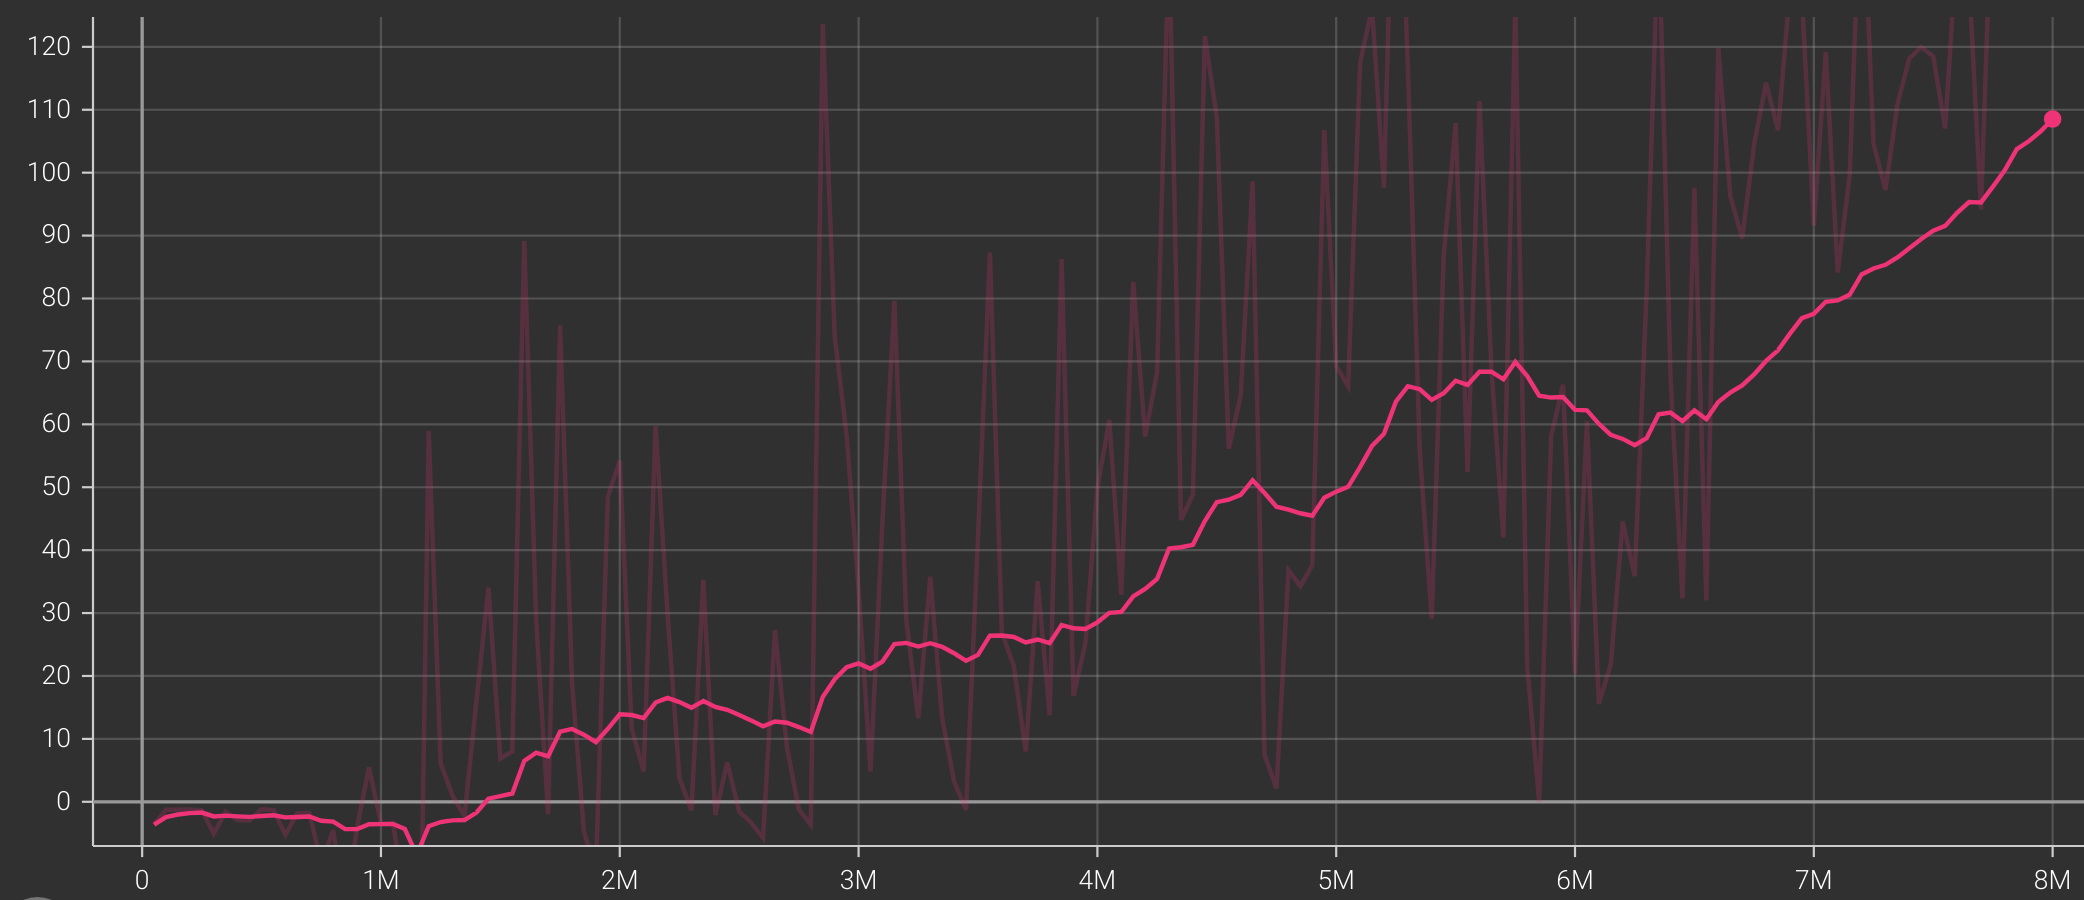
\includegraphics[width=1.0\textwidth]{images/graphs/AWS_baseline.png}
    \caption{\centering AWS Track Cumulative Reward. \\ X-axis: Time steps \\ Y-axis: Cumulative Reward}
    \label{fig:rl}
\end{figure}

\begin{figure}[H]
    \centering
    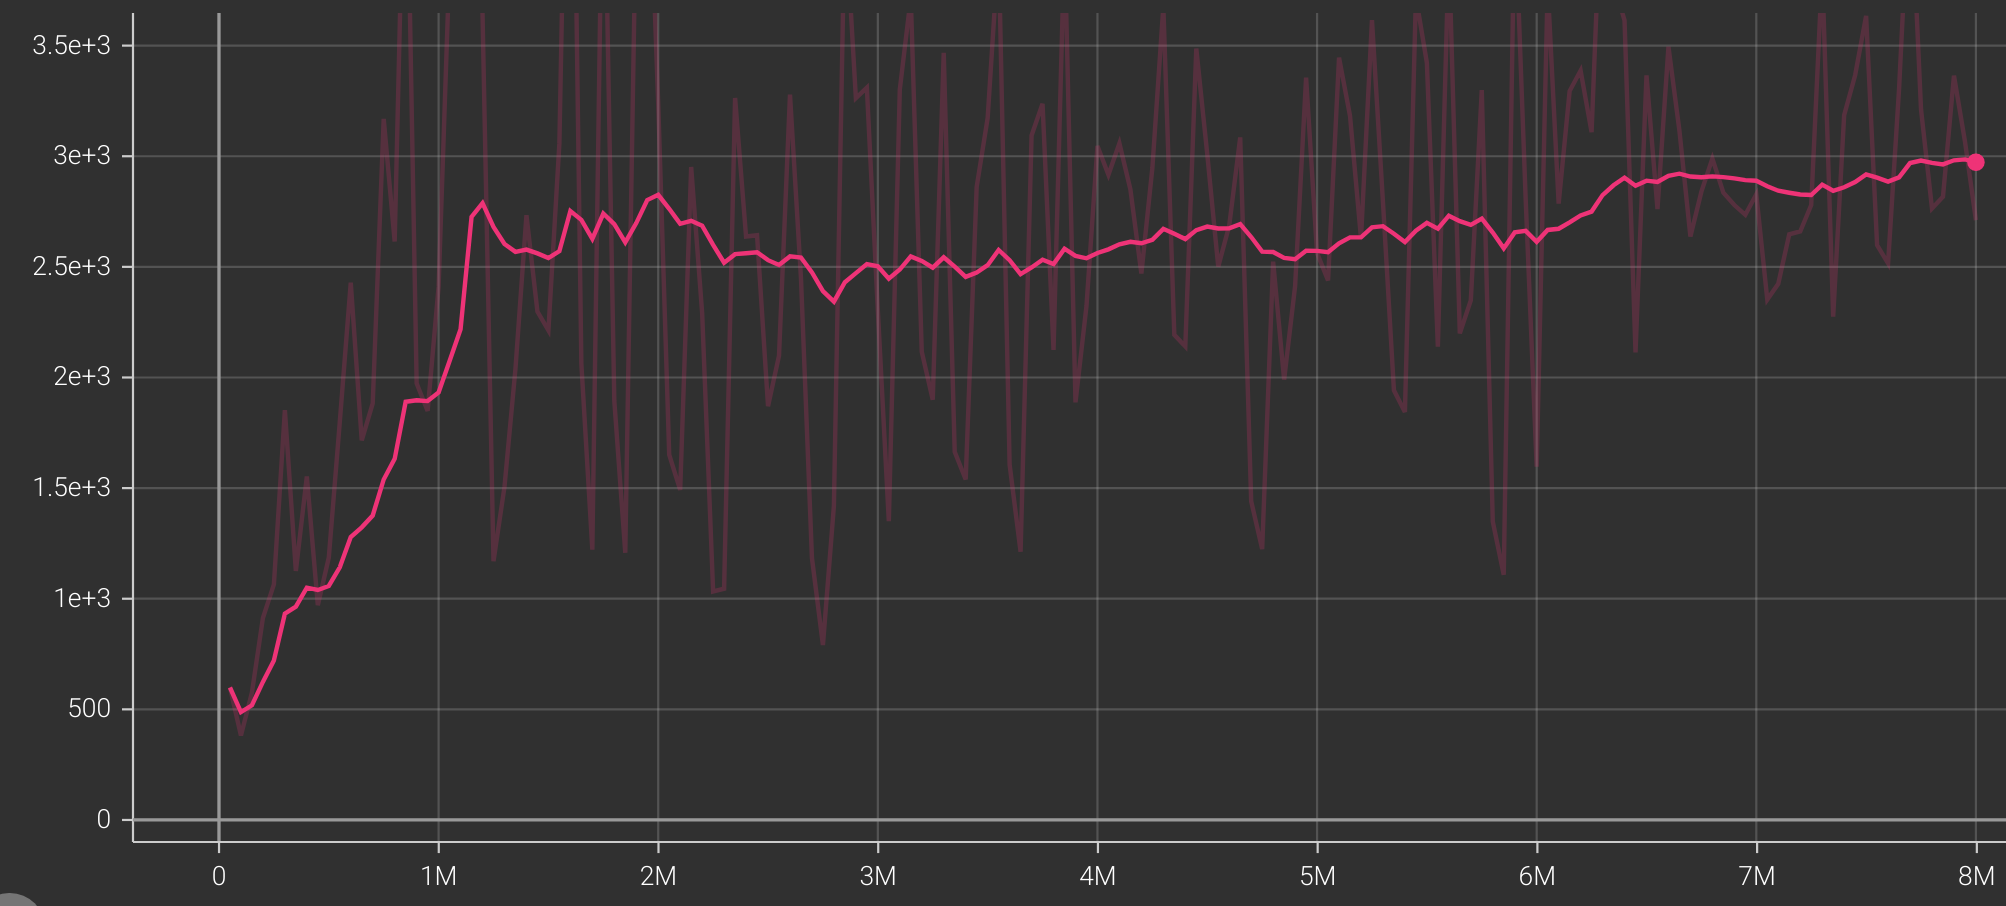
\includegraphics[width=1.0\textwidth]{images/graphs/AWS-EpisodeLength.png}
    \caption{\centering AWS Track Cumulative Reward. \\ X-axis: Time steps \\ Y-axis: Episode Length}
    \label{fig:rl}
\end{figure}

In this phase we record the baseline performance of the PPO algorithm on all the tracks that we have developed in table \ref{tab:baseline}. These scores will be used in the upcoming sections to quantify the effects and improvement of Transfer Learning and Adversarial Training.


\begin{table}[H]
\centering\begin{tabular}{|c|l|c|c|}
\hline
\textbf{Type}                                         & \textbf{Track} & \textbf{Steps (in Million)} & \textbf{Reward} \\ \hline
\multicolumn{1}{|c|}{\multirow{3}{*}{\textbf{Basic}}} & Oval Track     &  5                           &    41.2             \\ \cline{2-4} 
\multicolumn{1}{|c|}{}                                & One Kink       & 8                            &  90.7               \\ \cline{2-4} 
\multicolumn{1}{|c|}{}                                & Two Kink       & 8                           & 34.75           \\ \hline
\multirow{2}{*}{\textbf{Complex}}                     & Barcelona      & 12                         &   128.6              \\ \cline{2-4} 
                                                      & AWS Track      &        8                     & 136.8                 \\ \hline
\end{tabular}
\caption{Average reward scores of baseline models}
\label{tab:baseline}
\end{table}

\section{PHASE II - TRANSFER LEARNING}

\subsection{One Kink - Two Kink TL Performance}

Here we compare the performance obtained by model that uses transfer learning in comparison to the baseline model of the Two Kink track with the source track (One Kink) and target track (Two Kink) being tracks of the same class of complexity namely `Basic Tracks'.

\begin{figure}[H]
    \centering
    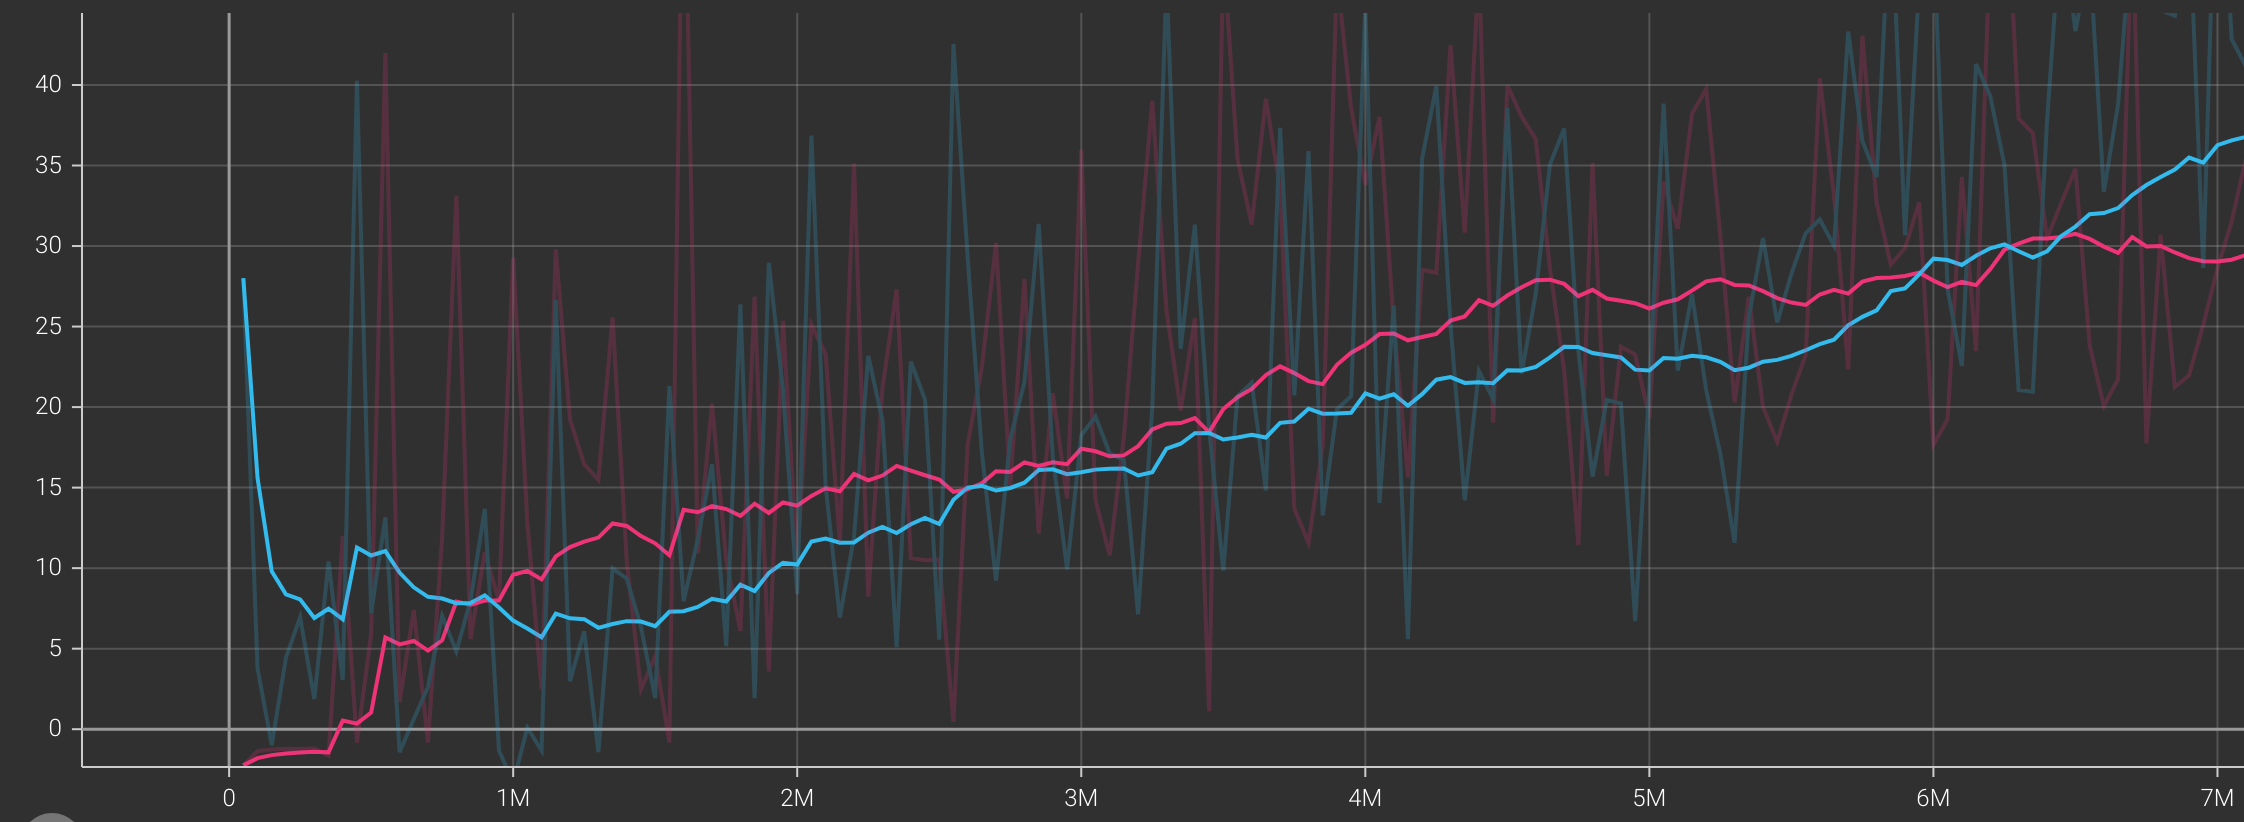
\includegraphics[width=1.0\textwidth]{images/graphs/TL-OneKink-TwoKink.png}
    \caption{\centering \textit{Blue}: Transfer Learned model, \textit{Pink}: Baseline model. \\ X-axis: Time steps \\ Y-axis: Cumulative Reward }
    \label{TL-OneKink-TwoKink}
\end{figure}
The graph in figure \ref{TL-OneKink-TwoKink} above represents the rewards obtained with Transfer Learning and without Transfer Learning on our Two Kink Track. The Transfer Learned model was trained first on the One Kink track for 1 Million steps and transferred for a further 7 Million steps on the Two Kink Track. Some key observations made are:
\begin{itemize}
\item The initial performance of the Transferred Model is higher as it has prior knowledge about the first few steps to be made which are track independent.
\item As the training further progresses, the scores obtained are very similar across both the models till the 6 Million step mark
\item The Transfer Learned model proceeds to performs better on the target task and achieves  13.1\% more reward(36.3 vs 32.1)  at the end of TL training.
\item While the results are positive, Transfer Learning in RL is still more volatile than in the case of DL and ML. This is further highlighted by the similar performance of the two models.
\end{itemize}


\subsection{Two Kink - AWS TL Performance}
In this experiment we perform transfer learning between tracks of two levels of complexity. Two Kink track is the most complex `Basic Track' and AWS track is the most complicated track that we use in our experimentation.
\begin{figure}[H]
    \centering
    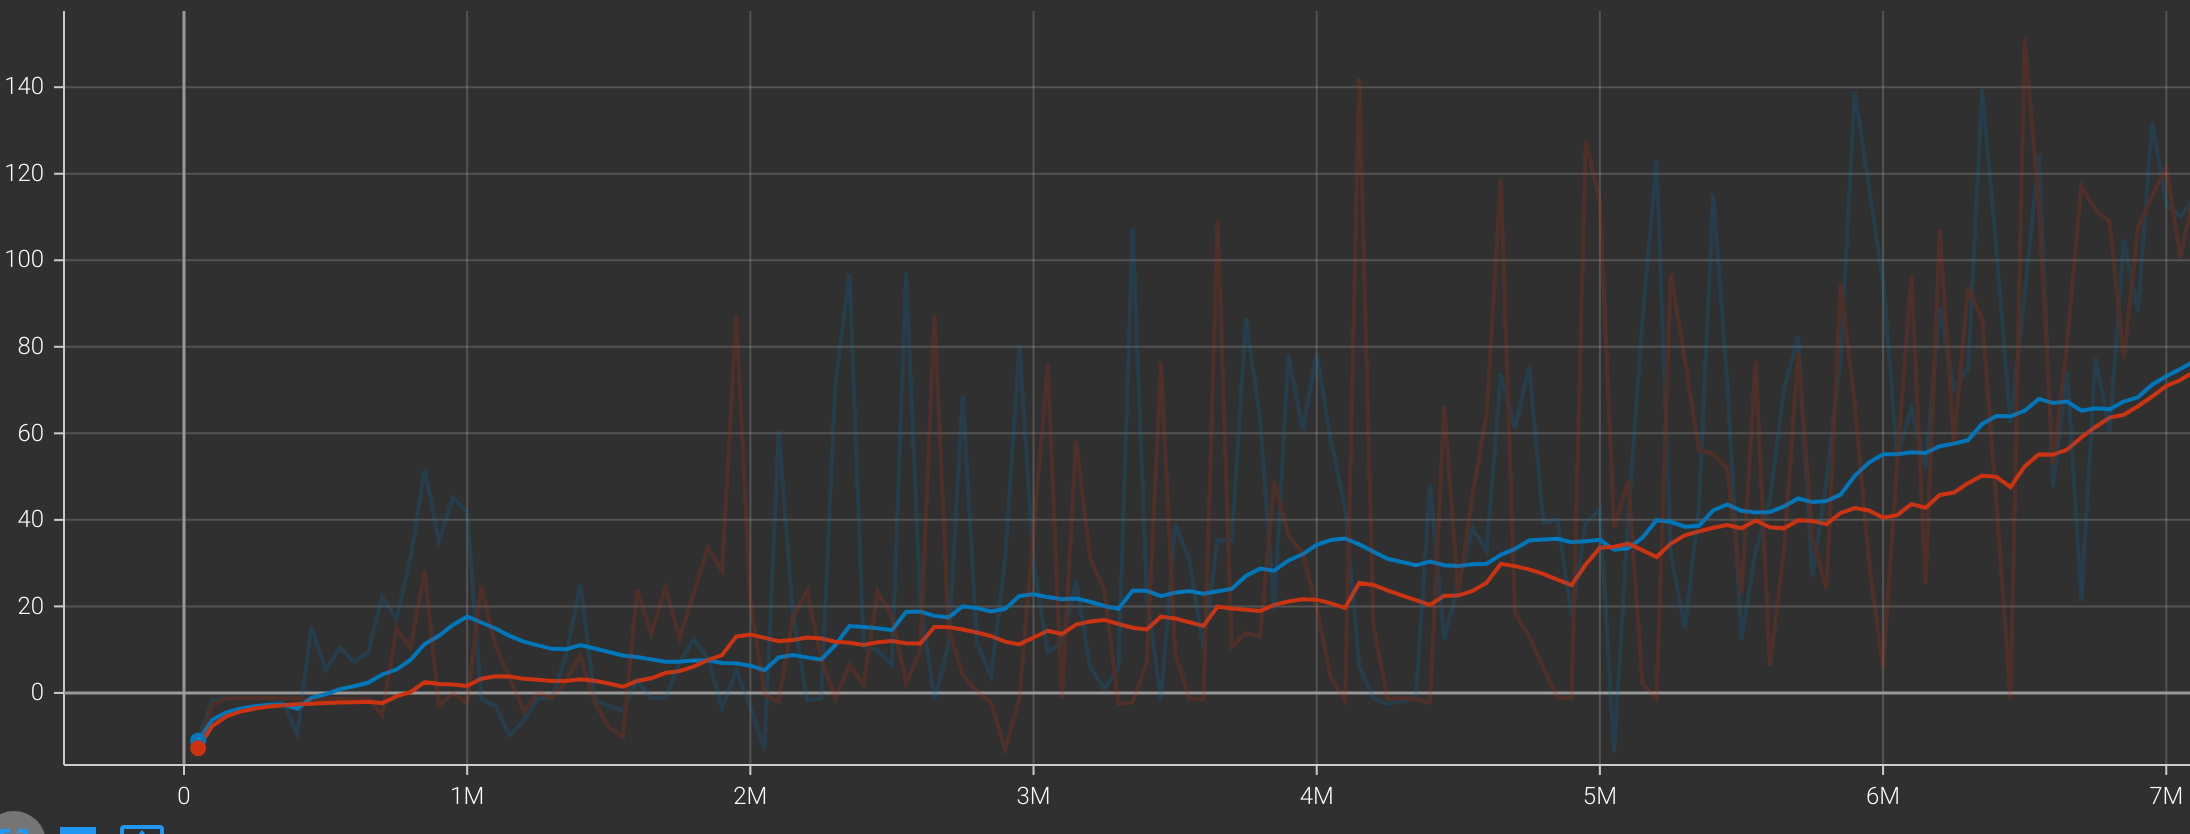
\includegraphics[width=1.0\textwidth]{images/graphs/TL-TwoKink-AWS.png}
    \caption{\centering \textit{Blue}: Transfer Learned model, \textit{Red}: Baseline model. \\ X-axis: Time steps \\ Y-axis: Cumulative Reward }
   
    
    \label{TL-TwoKink-AWS}
\end{figure}
The graph shown in figure \ref{TL-TwoKink-AWS} above represents the rewards obtained with Transfer Learning and without Transfer Learning on our AWS Track. The Transfer Learned model was trained first on the Two Kink track for 1 Million steps and transferred for a further 7 Million steps on the AWS Track. Some key observations made are:
\begin{itemize}
\item The performance of the Transfer Learned model is consistently around 5-7\% better than the baseline model from the start of training.
\item Around the 6.5 Million steps mark, the gap shrinks to a negligible difference with no significant improvement at the end of training
\end{itemize}

This further fortifies the findings that TL is much more challenging in RL than in DL or ML.


\section{PHASE III}


\subsection{Transfer Learning after Adversarial Training }
In this section we shall explore the effects and results of performing Adversarial Training. We shall discuss its effects on transfer learning between 2 tracks of similar complexity(One Kink track and Two Kink track), and between tracks of varying complexity(Two Kink Track and AWS Track).
We are using 2 different types of random noise attacks: Adversarial attack on the Observations(AT-TL) and the Adversarial Attack on the actions(AAT-TL)

\subsubsection{One Kink to Two Kink}

\begin{figure}[H]
    \centering
    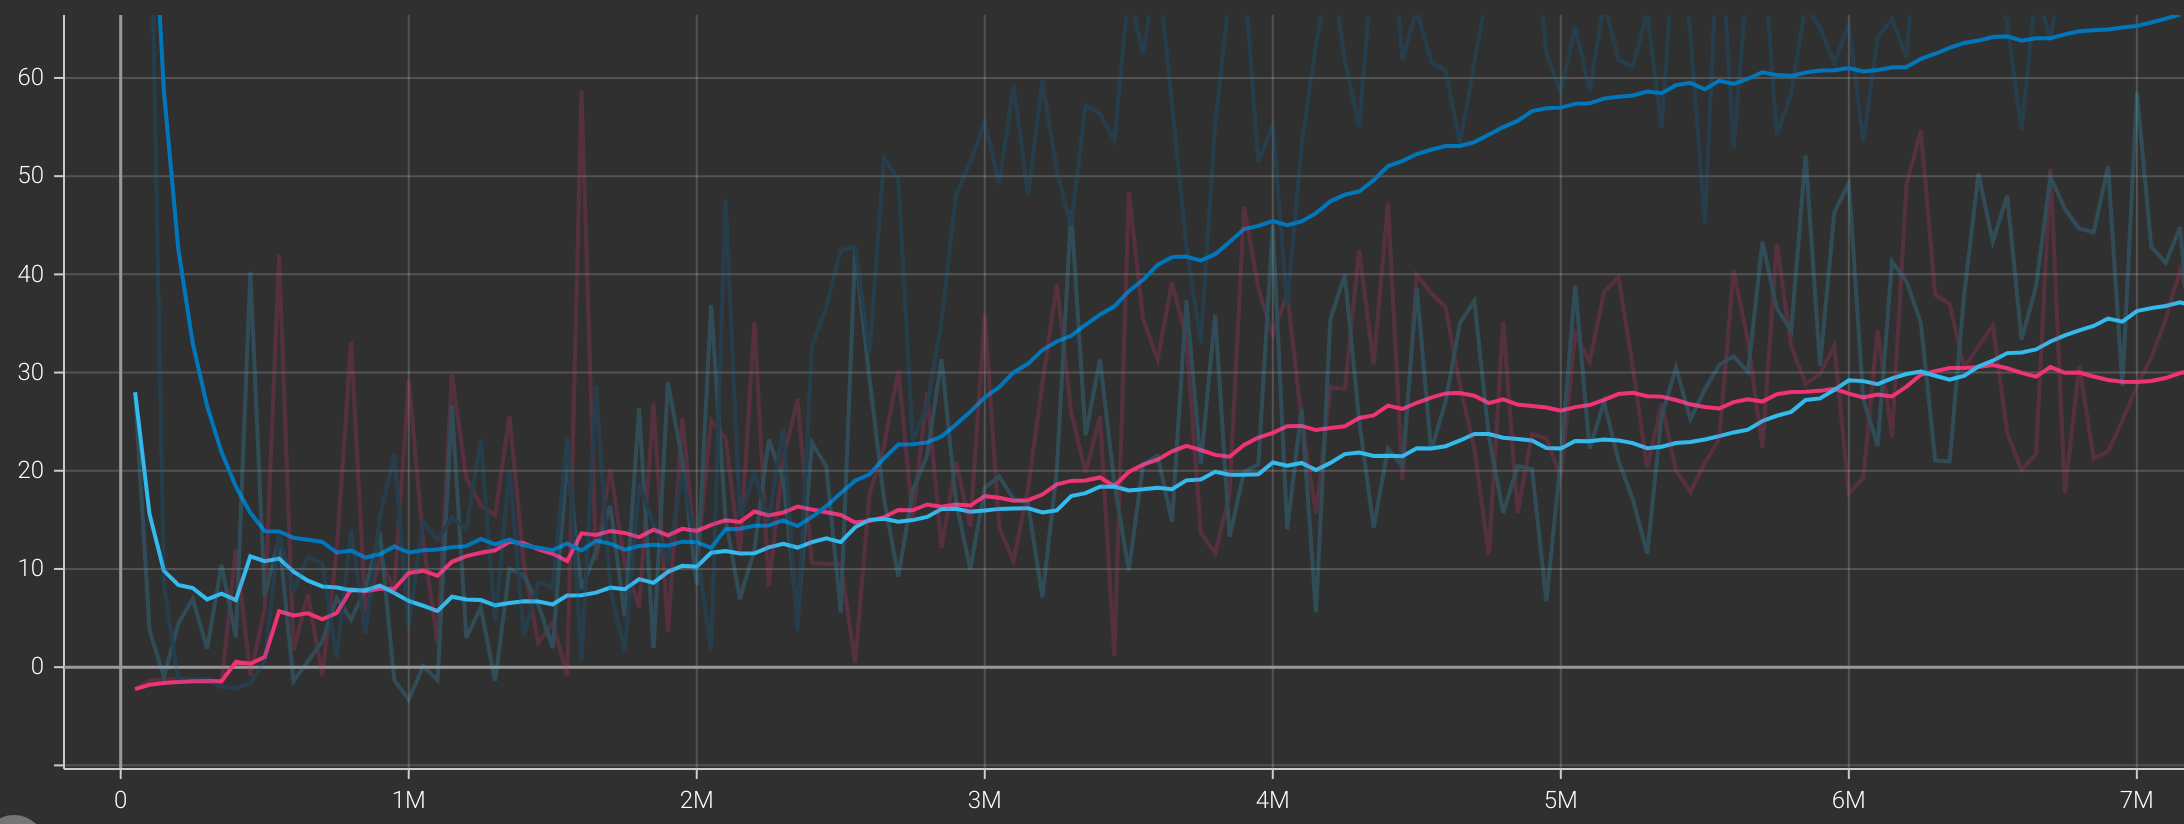
\includegraphics[width=1.0\textwidth]{images/graphs/AT-TL-OneKink-TwoKink.png}
    \caption{\centering \textit{Dark-Blue}: Adversarially Trained(Observation Attack) Transfer Learned model, \textit{Light-Blue}: Transfer Learned model, \textit{Red}: Baseline model. \\ X-axis: Time steps \\ Y-axis: Cumulative Reward }
   
    
    \label{fig:my_label}
\end{figure}

% The adversarial attack performed in this model is a random noise attack, which perturbs the sensory inputs of the model by moving the next checkpoint by a small distance.
% The above graph shows the model performance of the Adversarial trained - transfer learned model, compared to the simple transfer learned and baseline model. In this graph we can clearly see the advantage of using adversarial training. For the same number of steps the Adversarial trained model outperforms the other two models by a significant margin. 

\begin{figure}[H]
    \centering
    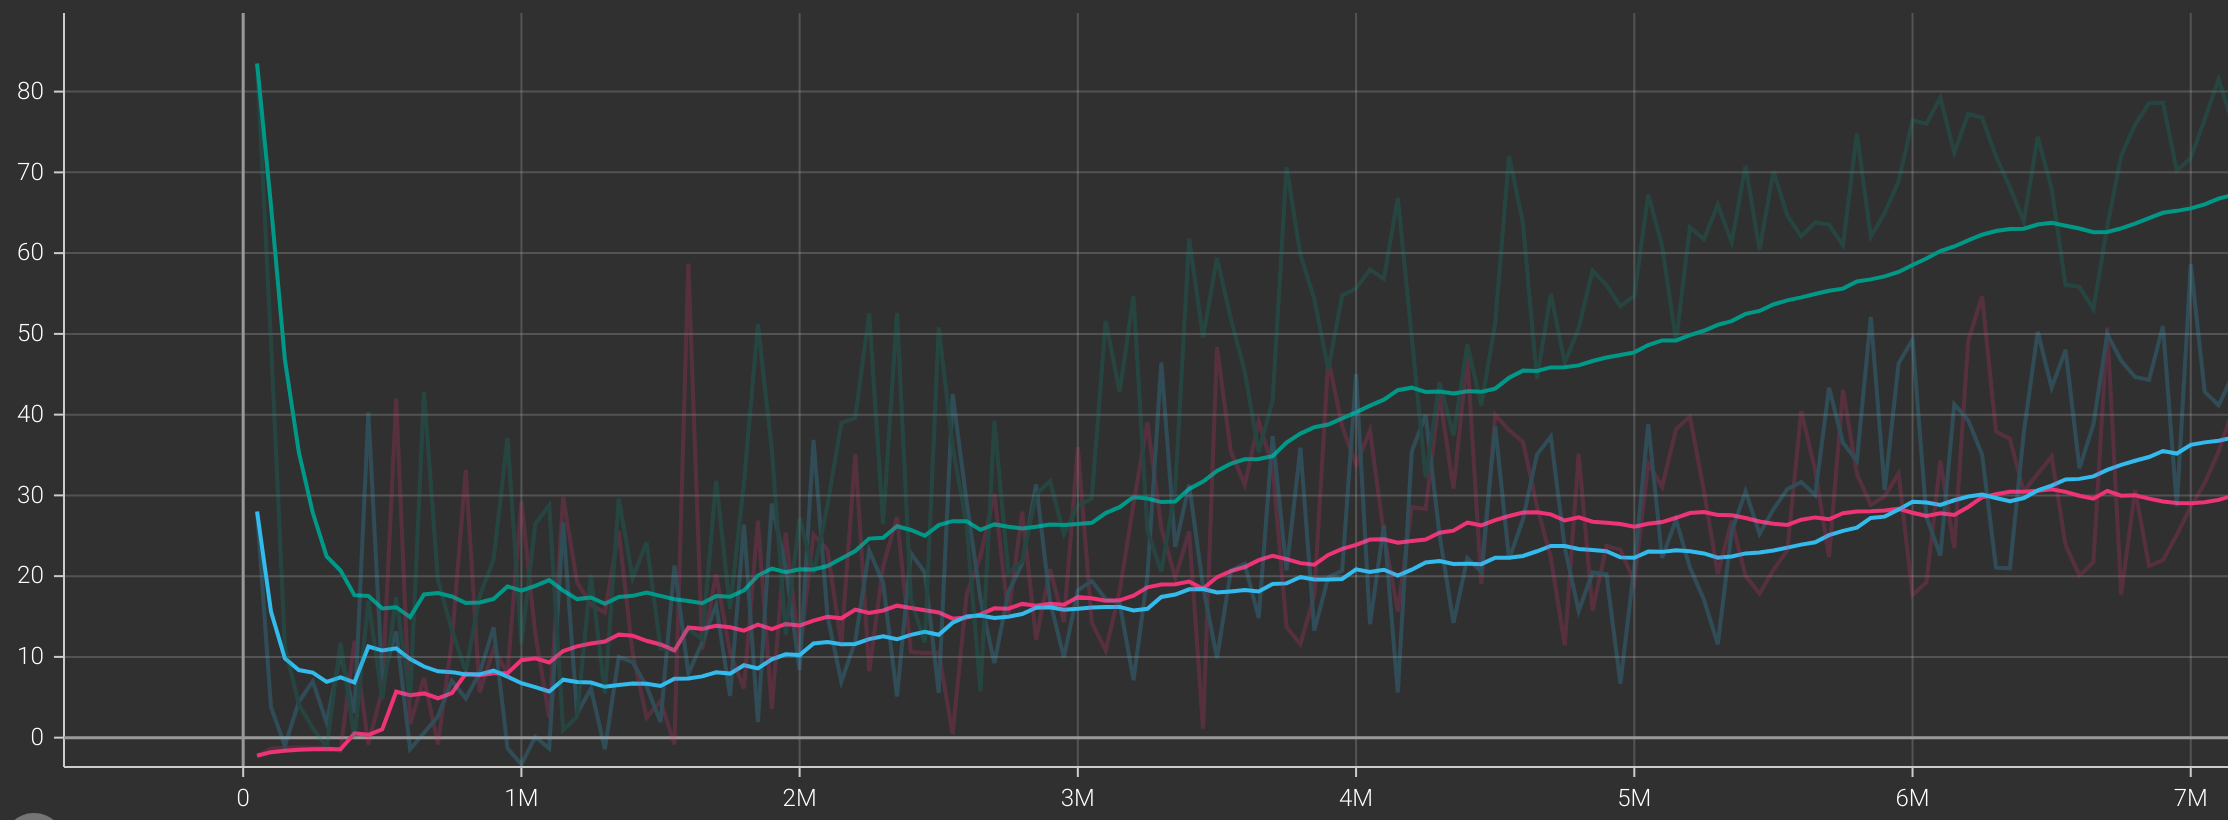
\includegraphics[width=1.0\textwidth]{images/graphs/AAT2-TL-OneKInk-TwoKink.png}
    \caption{\centering \textit{Green}: Adversarially trained(Action Attack) transfer learned model, \textit{Light-Blue}: Transfer Learned model, \textit{Red}: Baseline model. \\ X-axis: Time steps \\ Y-axis: Cumulative Reward }
   
    
    \label{fig:my_label}
\end{figure}

% This graph shows the performance of the model that is trained with an action adversary. Again we observe that the adversarial training followed by transfer learning improves the performance of the model/agent by a significant margin when compared to simple transfer learning.

% We can see that performing Adversarial Training followed by Transfer learning in both cases seems to be very effective; this may be attributed to the similarity of the layout of the tracks. The agent is able to better learn the state representations when we use adversarial training. The agent is able to use prior knowledge because of the higher quality of representations learned as a result of the adversarial training as we hypothesized. 

 Various Action Adversary Models were trained using different action adversary thresholds. It was observed that values between 0.2 to 0.5; we see a significant drop in performance when $threshold > 0.6$. 

\begin{itemize}
    \item The AT model reaches an average reward of 65.3 at 7 million steps, which is is significantly better than the Transfer Learning model (36.3).
    \item This is a 79.9\% improvement over the average reward obtained by the simple Transfer learned model
    \item We also observe that the AAT model is similar in performance to the AT model and reaches a score of 65.5 at the end of 7 million steps.
    \item This is again a 80.4\% improvement over the simple Transfer learned model.
\end{itemize}

We can see that performing Adversarial Training followed by Transfer learning in both cases seems to be extremely effective; this may be attributed to the similarity of the layout of the tracks. The agent is able to better learn the state representations when we use adversarial training and is thus performing better after transfer learning.


\subsubsection{Two Kink to AWS }

\begin{figure}[H]
    \centering
    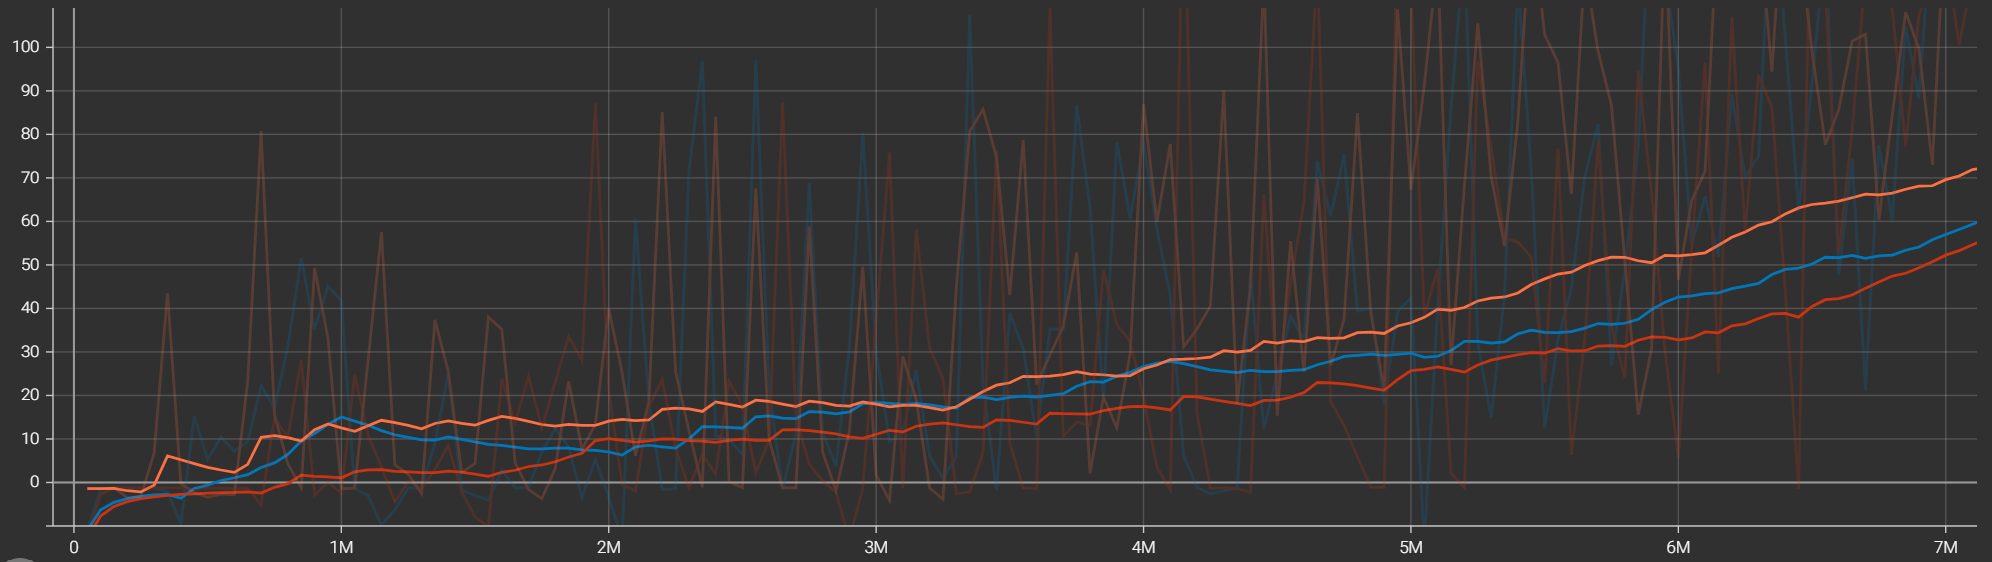
\includegraphics[width=0.9\textwidth]{images/graphs/AT-TL-TwoKink-AWSTrack-0.98.png}
    \caption{\centering \textit{Orange}: Adversarially Trained(Observation Attack) Transfer Learned model, \textit{Blue}: Transfer Learned model, \textit{Red}: Baseline model. \\ X-axis: Time steps \\ Y-axis: Cumulative Reward }
   
    
    \label{fig:my_label}
\end{figure}

% In this graph we can observe that the results produced by the observation adversary trained transfer learned model(AT-TL) performs better that the baseline model and the transfer learned model. The AT-TL model uses adversarial training that disrupts


\begin{figure}[H]
    \centering
    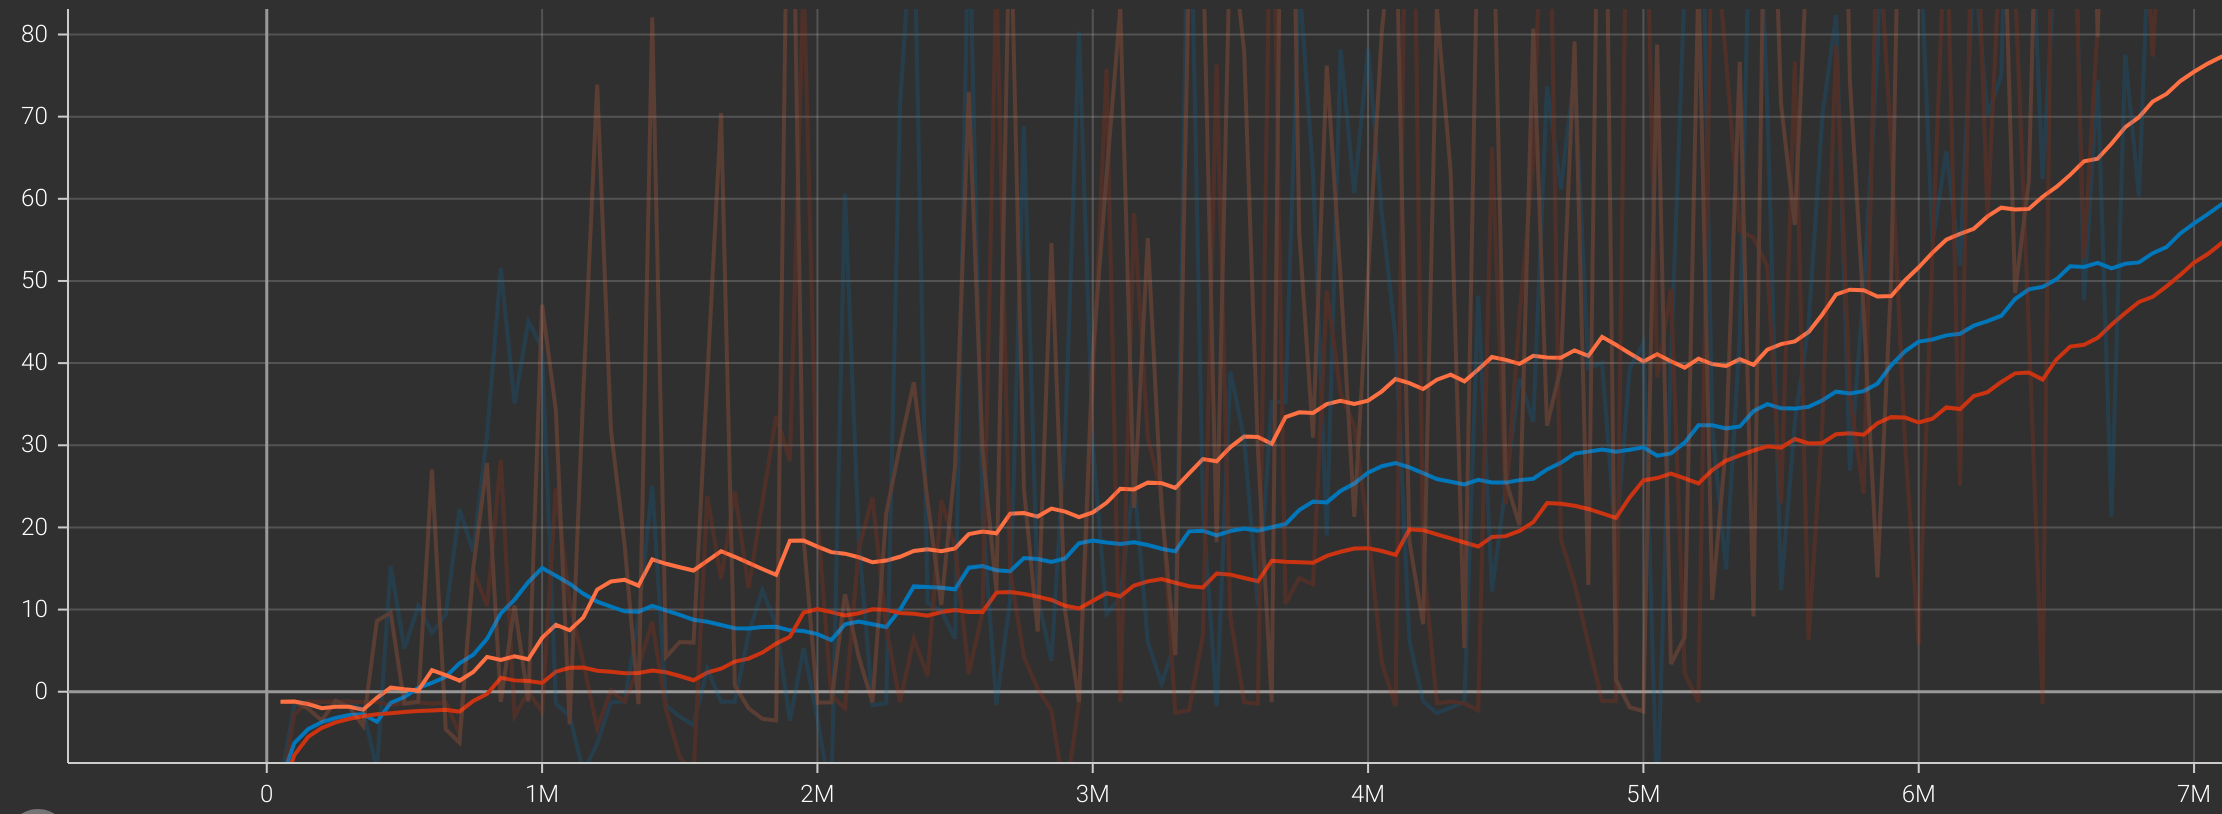
\includegraphics[width=0.9\textwidth]{images/graphs/AAT2-TL-TwoKink-AWS.png}
    \caption{\centering \textit{Orange}: Adversarially Trained(Action Attack) Transfer Learned model, \textit{Blue}: Transfer Learned model, \textit{Red}: Baseline model. \\ X-axis: Time steps \\ Y-axis: Cumulative Reward }
   
    
    \label{fig:my_label}
\end{figure}

\begin{itemize}
    \item The AT-TL model achieve a score of 69.6 and the AAT-TL model achieves a score of 75.5 at the end of 7 million steps.
    \item The AT-TL model gives us an improvement of 21.9\% over the TL model and similarly the AAT-TL model gives us an improvement of 32.2\%.
    \item Given the stark differences in complexity of the Two Kink Track and the AWS Track, this improvement in performance is a significant improvement over the results seen when performing vanilla transfer learning.
\end{itemize}

 

% \begin{table}[H]
% \begin{tabular}{|l|l|l|}
% \hline
% \textbf{Model}                      & \textbf{Steps (in millions)} & \textbf{Average Reward} \\ \hline
% TL Model OneKink - TwoKink & 8                   & 39.7           \\ \hline
% TL - AT OneKink - TwoKink  & 8                   & 69.8           \\ \hline
% TL - AAT OneKink - TwoKink & 8                   & 63.9           \\ \hline
% TL Model TwoKink - AWS     & 7                   & 57.1               \\ \hline
% TL - AT TwoKink - AWS      & 7                   & 69.6             \\ \hline
% TL - AAT TwoKink - AWS     & 7                   & 75.5             \\ \hline
% \end{tabular}
% \end{table}
Table \ref{tab:phase2} shows the consolidated results obtained across Phase 2 and Phase 3 of our experimentation.

\begin{table}[H]
\begin{tabular}{|p{1.8cm}|p{1.8cm}|l|p{1.8cm}|l|p{3.2cm}|}
\hline
\textbf{Source Track} & \textbf{Target Track} & \textbf{Training Type} & \textbf{Steps ($\times 10^{6}$)} & \textbf{Average Reward} & \textbf{\%improvement (wrt TL)} \\ \hline
\multirow{3}{*}{OneKink}               & \multirow{3}{*}{TwoKink}               & TL                                      & 7                                             & 36.3                                     & -                      \\ \cline{3-6} 
                                      &                                        & AT - TL                                 & 7                                             & 65.3                                     & 79.9                   \\ \cline{3-6} 
                                      &                                        & AAT - TL                                & 7                                             & 65.5                                     & 80.4                   \\ \hline
\multirow{3}{*}{TwoKink}               & \multirow{3}{*}{AWS}                   & TL                                      & 7                                             & 57.1                                     & -                      \\ \cline{3-6} 
                                      &                                        & AT - TL                                 & 7                                             & 69.6                                     & 21.9                   \\ \cline{3-6} 
                                      &                                        & AAT - TL                                & 7                                             & 75.5                                     & 32.2                   \\ \hline
\end{tabular}
\caption{Average reward  of different Adversarial Attacks and Transfer Learned Models \\ AT - Observation Attack \\ AAT - Action Attack}
\label{tab:phase2}
\end{table}


% \begin{table}[H]
% \centering\begin{tabular}{|l|l|l|c|p{2.5cm}|}
% \hline
% \textbf{Source Track}             & \textbf{Target Track}             & \textbf{Training Type} & \textbf{Steps (in millions)} & \textbf{Average Reward} \\ \hline
% \multirow{3}{*}{OneKink} & \multirow{3}{*}{TwoKink} & TL            & 7                   & 36.3           \\ \cline{3-5} 
%                          &                          & AT - TL       & 7                   & 65.3            \\ \cline{3-5} 
%                          &                          & AAT - TL      & 7                   & 65.5           \\ \hline
% \multirow{3}{*}{TwoKink} & \multirow{3}{*}{AWS}     & TL            & 7                   &  57.1               \\ \cline{3-5} 
%                          &                          & AT - TL       & 7                   &      69.6         \\ \cline{3-5} 
%                          &                          & AAT - TL      & 7                   &       75.5         \\ \hline
% \end{tabular}
% \caption{Average reward  of different Adversarial Attacks and Transfer Learned Models \\ AT - Observation Attack \\ AAT - Action Attack}
% \label{tab:phase2}
% \end{table}